\subsection{Overview}

Since planning for different kits is a major problem area in building a
flexible kitting workstation, the authors are focusing on planning for
kitting.  A test method is being developed that will be suitable for
comparing the performance of different kitting planning systems.  To build
such a test method, representations for three sets of data are needed:
\begin{itemize}
\item a representation for the initial conditions in the kitting workstation
 from which planning starts (the initial state)

\item a representation for the desired final conditions in the kitting 
workstation after the plan has been executed (the goal state)

\item a representation for a plan to get from the initial state to the goal
state.
\end{itemize}

The first two representations are of the same nature: a description
primarily of objects and their locations. Hence, the same representation
may be used for both. Details follow shortly.

The representation of a plan is of a different nature. A plan is primarily
a description of actions that change one kitting workstation state to
another. Since the only active element in the model of a kitting
workstation is a one-armed robot, the plan model is a sequential
list of actions for a robot to perform.

\subsection{Kitting Workstation Model}

Conceptually, the kitting workstation model is an object model as found in
several object oriented programming languages (C++, for example
\cite{Stroustrup.2000}).  That is:
\begin{itemize}
\item the model consists primarily of class definitions
\item a class defines a type of thing
\item classes have attributes (``elements'' in XML schema language)
\item the class definition gives the class (or data type) of each attribute
\item some attributes may occur optionally or multiple times
\item some classes are derived from others; thus, there is a derivation
 hierarchy 
\item a derived class has all the attributes of its parent plus, possibly,
  some of its own
\item if class B is derived from class A, then if the type of an attribute
  is class A, an instance of class B may be used as the value of the attribute
\item the model does not use multiple inheritance
\item the model also uses primitive data types such as numbers and strings
  and provides for defining specialized data types by putting constraints
  on primitive data types.
\end{itemize}

A complete hierarchical list of the classes used in the kitting workstation
model is shown in Figure~\ref{fig:ClassHierarchy}. In the list, there are two
top-level classes, SolidObject and DataThing. All other classes are
derived. Each class that is indented in the list is derived from the first
less indented class above it. For example, PartsBin is derived from
BoxyObject, and BoxyObject is derived from SolidObject. The figure does not
show any attributes.

\begin{figure}[ht]
\fbox{
\begin{minipage}{3.2in}
\tt
\begin{tabbing}
xx\=xx\=xx\=\kill
SolidObject\\
\>BoxyObject\\
\>\>KitTray\\
\>\>LargeContainer\\
\>\>PartsBin\\
\>\>PartsTray\\
\>\>WorkTable\\
\>EndEffector\\
\>\>GripperEffector\\
\>\>VacuumEffector\\

\>\>\>VacuumEffectorMultiCup\\
\>\>\>VacuumEffectorSingleCup\\
\>EndEffectorHolder\\
\>Kit\\
\>KittingWorkstation\\
\>LargeBoxWithEmptyKitTrays\\
\>LargeBoxWithKits\\
\>Part\\
\>PartsTrayWithParts\\
\>Robot\\
DataThing\\
\>BoxVolume\\
\>KitDesign\\
\>PartRefAndPose\\
\>PhysicalLocation\\
\>\>PoseLocation\\
\>\>\>PoseLocationIn\\
\>\>\>PoseLocationOn\\
\>\>\>PoseOnlyLocation\\
\>\>RelativeLocation\\
\>\>\>RelativeLocationIn\\
\>\>\>RelativeLocationOn\\
\>Point\\
\>ShapeDesign\\
\>StockKeepingUnit\\
\>Vector\\
\end{tabbing}
\rm
\caption{Kitting Workstation Model Class Hierarchy}
\label{fig:ClassHierarchy}
\end{minipage}
}
\end{figure}

The structure of the kitting workstation class (or type) is shown in
Figure~\ref{fig:WorkstationModel}. The figure shows the names of the
attributes of a kitting workstation. The first three attributes (Name,
PrimaryLocation and SecondaryLocation) are inherited from the SolidObject
class. The rest of the attributes are specific to the kitting workstation
class. The AngleUnit, LengthUnit, and WeightUnit apply to all quantities in
a data file that are in terms of those unit types. No other unit types are
used in the model.

In Figure~\ref{fig:WorkstationModel} and similar figures (which were
generated by XMLSpy from XML schemas), a dotted line around a box
means the attribute is optional (may occur zero times), while a \sf
..infinity \rm underneath a box means it may occur more than once, with no
upper limit on the number of occurrences.

\begin{flushleft}
\fbox{
\begin{minipage}[t]{3.17in}
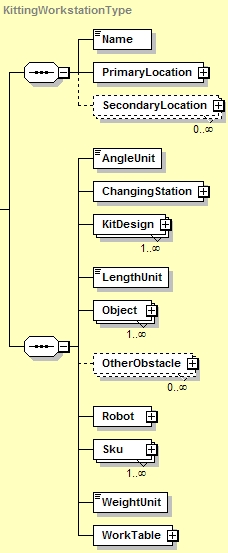
\includegraphics[width=3.166in]{images/kittingModelSmallCropped.jpg}
\end{minipage}
}
\end{flushleft}

\begin{figure}[h]
\caption{Kitting Workstation Model}
\label{fig:WorkstationModel}
\end{figure}

The types (i.e. classes or datatypes) of the attributes of a kitting
workstation are not shown on Figure~\ref{fig:WorkstationModel}. The
structures of several of the attributes are shown on the following figures:
\begin{itemize}
\item ChangingStation -- EndEffectorChangingStationType:
  Figure~\ref{fig:ChangingStation}
\item KitDesign -- KitDesignType: Figure~\ref{fig:KitDesign}
\item Object -- LargeBoxWithEmptyKitTraysType Figure~\ref{fig:LBWEKT},
  LargeBoxWithKitsType Figure~\ref{fig:LBWK}, and PartsTrayWithParts
  Figure~\ref{fig:PTWP}
\item Robot -- RobotType Figure~\ref{fig:Robot}
\item Sku -- StockKeepingUnitType Figure~\ref{fig:SKU}
\item WorkTable -- WorkTableType Figure~\ref{fig:WorkTable}.
\end{itemize}

The type of the Object elements of a kitting workstation is
SolidObject. That is an abstract class not intended to be
instantiated. Hence, the figures show the structures of derived classes of
SolidObject that are intended to be used for instances of the Object
attribute.

\begin{flushleft}
\fbox{
\begin{minipage}[t]{3.17in}
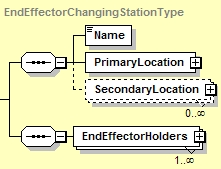
\includegraphics[width=3.166in]{images/changingStation.jpg}
\end{minipage}
}
\end{flushleft}
\begin{figure}[h]
\caption{Changing Station Model}
\label{fig:ChangingStation}
\end{figure}

\begin{flushleft}
\fbox{
\begin{minipage}[t]{3.17in}
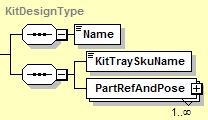
\includegraphics[width=3.1in]{images/kitDesign.jpg}
\end{minipage}
}
\end{flushleft}
\begin{figure}[h]
\caption{Kit Design Model}
\label{fig:KitDesign}
\end{figure}

\begin{flushleft}
\fbox{
\begin{minipage}[t]{3.17in}
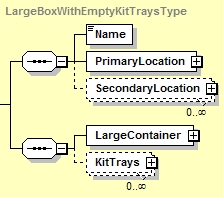
\includegraphics[width=3.1in]{images/largeBoxWithEmptyKitTrays.jpg}
\end{minipage}
}
\end{flushleft}
\begin{figure}[h]
\caption{Large Box With Empty Kit Trays Model}
\label{fig:LBWEKT}
\end{figure}

\begin{flushleft}
\fbox{
\begin{minipage}[t]{3.17in}
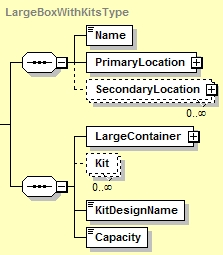
\includegraphics[width=3.1in]{images/largeBoxWithKits.jpg}
\end{minipage}
}
\end{flushleft}
\begin{figure}[h]
\caption{Large Box With Kits Model}
\label{fig:LBWK}
\end{figure}

\begin{flushleft}
\fbox{
\begin{minipage}[t]{3.17in}
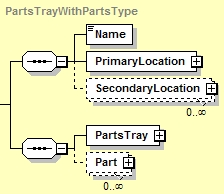
\includegraphics[width=3.1in]{images/partsTrayWithParts.jpg}
\end{minipage}
}
\end{flushleft}
\begin{figure}[h]
\caption{Parts Tray With Parts Model}
\label{fig:PTWP}
\end{figure}

\begin{flushleft}
\fbox{
\begin{minipage}[t]{3.17in}
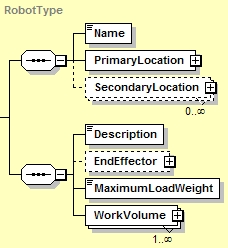
\includegraphics[width=3.166in]{images/robot.jpg}
\end{minipage}
}
\end{flushleft}
\begin{figure}[h]
\caption{Robot Model}
\label{fig:Robot}
\end{figure}

The robot model is simple and does not currently have any kinematics or
even any shape for the robot. It is likely that additional attributes will
be added in the future.

\begin{flushleft}
\fbox{
\begin{minipage}[t]{3.17in}
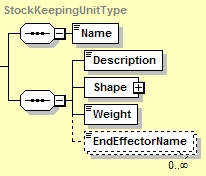
\includegraphics[width=3.166in]{images/sku.jpg}
\end{minipage}
}
\end{flushleft}
\begin{figure}[h]
\caption{Stock Keeping Unit Model}
\label{fig:SKU}
\end{figure}

\begin{flushleft}
\fbox{
\begin{minipage}[t]{3.17in}
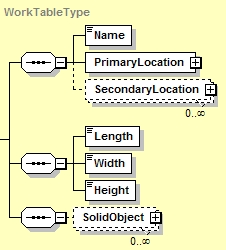
\includegraphics[width=3.166in]{images/worktable.jpg}
\end{minipage}
}
\end{flushleft}
\begin{figure}[h]
\caption{Work Table Model}
\label{fig:WorkTable}
\end{figure}

The kitting workstation model has been fully defined in each of two
languages: XML schema language \cite{Walmsley.2002},
\cite{XMLschemaPrimer}, \cite{XMLschemaStructures}, and Web Ontology
Language (OWL \it sic\rm) \cite{OWLoverview}, \cite{OWLprimer},
\cite{OWLspec}. Although the two models are conceptually identical, there
are some systematic differences between the models (in addition to
differences inherent in using two different languages).

\begin{itemize}

\item The complexType names (i.e. class names) in XML schema have the
  suffix ``Type'' added which is not used in OWL. This is so that the same
  names without the suffix can be used in XML schema language as element
  names without confusion.

\item All of the XML schema complexTypes have a ``Name'' element that is
  not present in OWL. It is not needed in OWL because names are assigned as
  a matter of course when instances of classes are created.

\item The movable objects that are in the kitting workstation are
  explicitly modeled in the XML schema model but not in the OWL model.

\item Attribute names in OWL have a prefix, as described below. The
  prefixes are not used in XML schema.

\end{itemize}

\subsection{Using OWL}

The kitting workstation model was defined first in OWL because the IEEE RAS
Ontologies for Robotics and Automation Working Group has decided to use
OWL, and the authors are participating in the activities of that working
group. OWL allows the use of several different syntaxes. The
functional-style syntax (which is the most compact one) has been used to
write the OWL version of the kitting workstation model.

In addition to having the model defined in OWL, OWL data files describing
specific initial states and goal states were defined in OWL, also using the
functional-style syntax.  Software tools were built in C++ to work with the
OWL model and data files conforming to the model.

The initial intent has been to use OWL files for presenting the initial and
goal conditions for planning problems, and the authors have implemented a
planning system that uses OWL files.

The primary tool used by the OWL community for building and checking OWL
models and data files is named Protege \cite{Horridge.2011}. Protege was
used for checking the kitting model and data files as they were
built. Protege continues to be used for checking the model and data files
whenever they are changed. The layout of the hierarchy in
Figure~\ref{fig:ClassHierarchy} is identical to what may be seen in
Protege's class hierarchy window when the kitting model is loaded (but
Protege makes it look better).

Several difficulties of working with OWL were encountered. The primary
effect of these difficulties was to make it essentially impossible to
debug OWL files.

Defining a model in OWL is quite different from defining the same model in
other information modeling languages with which the authors are intimately
familiar: C++, EXPRESS \cite{EXPRESSmanual}, and XML schema. Three of the
major differences involve (1) the assignment of attributes in classes, (2)
OWL's ``open world'' assumption, and (3) the distinction between model
files and data files.\\

\subsubsection{Class Attributes}

In other languages, assigning a typed attribute to a class requires a
single line of code. For example, the X attribute may be put into a
cartesian point class in XML schema language with
\newline \sf $<$xs:element name=``X'' type=``xs:decimal''/$>$\rm
\newline or in C++ with
\newline \sf double X; \rm
\newline or in EXPRESS with
\newline \sf X : REAL; \rm \newline
In these other languages, the name of the attribute is local to the class.
Hence, an attribute with a given name can appear in more than one class, and
there will be no confusion.

In OWL, there is no simple method of declaring a class attribute. Instead,
a property must be declared along with properties of the property. The
following lines are used in the OWL model to say that all points and only
points have an X attribute which is a decimal number.
\newline
\newline \sf Declaration(DataProperty(hasPoint\_X))
\newline DataPropertyDomain(:hasPoint\_X :Point)
\newline DataPropertyRange(:hasPoint\_X xsd:decimal)
\newline EquivalentClasses(:Point ObjectIntersectionOf(
\newline \hspace*{0.2in}DataSomeValuesFrom(:hasPoint\_X xsd:decimal)
\newline \hspace*{0.2in}DataAllValuesFrom(:hasPoint\_X xsd:decimal))) \rm
\newline
\newline
The \sf hasPoint \rm prefix used in the property name is not an OWL
requirement. It is one of several naming conventions for OWL being used by
the authors. The prefix is both for the benefit of a human reader (to make
it obvious that this is a property of a Point) and to differentiate this X
attribute from an X attribute of some other class (call it \sf Foo\rm)
which would have the prefix \sf hasFoo \rm.

As described above, with OWL, it is necessary to make many statements in
order to build a class in a typical object-oriented style. OWL does not
assume a typical object-oriented style. It assumes the world might be more
complex than that. Hence, many OWL statements are required to produce
effects made in a few statements in other object-oriented languages. Having
to write a lot of statements is tedious but not a roadblock. A more serious
problem is that if a statement necessary to produce an object-oriented
effect is omitted, that is not an OWL error. Protege does not have an
object-oriented mode in which it will warn the user if a required statement
is missing. There are no OWL tools that will help with finding missing
statements. This is a debugging problem.

OWL was built so that it would support automated reasoning about the
relationships among properties, classes, and individuals. Protege allows
the use of several alternate automatic reasoners. In a typical
object-oriented style, there is no use for reasoning of that sort.
Everything useful to know about the relationships among properties,
classes, and individuals is already known. Hence having an automated
reasoning capability of the sort for which OWL was built is not useful
for the kitting model.\\

\subsubsection{Open World Assumption}

OWL makes an ``open world'' assumption.  In an open world, anything might
be true that is not explicitly declared false and is not inconsistent with
what has been declared true. This makes it easy for errors to go
unrecognized as such by Protege (or any other OWL tool). For example,
suppose the line \sf DataPropertyDomain(:hasPoint\_X :Point) \rm given
above is mistyped as \sf DataPropertyDomain(:hasPoint\_x :Point) \rm. When
Protege loads the file and the reasoner is started, no errors are
detected. Protege assumes that the DataPropertyDomain for \sf hasPoint\_X
\rm is unknown (that's fine in OWL and Protege) and that there is a new
property named \sf hasPoint\_x \rm about which the only thing known is its
DataPropertyDomain (also fine in OWL and Protege, even though there is no
explicit DataProperty declaration for the new property). The error can be
detected by a human by studying the list provided by selecting the
DataProperties tab in Protege, but the human should not have to go to such
lengths. Similar errors, such as mistyping the name of an individual, are
similarly accepted in OWL and Protege as being OK, with similar effects.
The difficulties caused by the open world assumption would not occur if
Protege had a closed world mode, but it has none.\\

\subsubsection{Model Files vs. Data Files}

While other languages have different file formats for models and
data conforming to the models, OWL does not distinguish between model files
and data files. Protege does not provide any method of specifying that a
file is a model file or a data file. The conceptual difference is simple,
even in OWL. Model files describe classes and data types (and, possibly,
constraints). Data files give information about individuals (instances of
one or more classes -- often called objects). The authors have made it a
practice to distinguish OWL model files from OWL data files. An OWL data
file can inadvertently change an OWL model, a bug that is very hard to
find. That cannot happen with EXPRESS or XML schema.\\

\subsubsection{Bugs in Files}

Since humans are error-prone, and the kitting OWL files were built by
humans, the OWL files had errors of the sort mentioned above. Some of these
errors were discovered when the OWL files were processed by the tools
developed for processing them and strange results were observed. Other
errors were found when a method of generating OWL data files automatically
from XML data files was developed, as described next.

\subsection{Using XML Schema and XML Data Files}

To work around the difficulties of using OWL while continuing to use OWL,
the authors are using XML schema and XML data files in parallel with the
corresponding OWL files.\\

\subsubsection{XML Tools}

Two automated tools developed by the authors are being used: an xml schema
parser (xmlSchemaParser) and a code generator (GenXMiller).  Neither of
these has yet been documented elsewhere.

The xmlSchemaParser reads an XML schema file, stores it in terms of
instances of C++ classes, and reprints the schema. When the xmlSchemaParser
runs, it performs many checks on the validity of the schema that is input
to it. The xmlSchemaParser handles almost all portions of the XML schema
syntax. A few of the rarely-used bits of syntax are not implemented.

The GenXMiller reads an XML schema and writes code for reading and writing
XML data files corresponding to that schema. The code that is generated
includes C++ classes (.hh and .cc files), a parser (YACC and Lex files) and
a stand-alone parser file in C++ that uses the other files.  The executable
utility produced by compiling a stand-alone parser reads and echos any XML
data file corresponding to the schema. The GenXMiller is still under
development. It handles many schemas, but has not implemented enough of
the XML schema language to handle many others. The GenXMiller is not a
new type of system. Several other code generators that use an XML schema
as input have been developed. Even more XML schema parsers are
available. However, having the knowledge about XML schema and XML data
files gained by developing that software and having an intimate knowledge
of the source code for it has proved very valuable in using XML to deal
with OWL.

The xmlSchemaParser and the GenXMiller use the same underlying parser,
which is built in YACC and Lex \cite{LexAndYACC}.

In addition to using the xmlSchemaParser and the GenXMiller, a commercial
XML tool named XMLSpy \cite{XMLSpyManual} has been used to check all XML
schemas and XML data files.\\

\subsubsection{Handling Kitting Data Files}

There is only one conceptual kitting model but there are several kitting
data files corresponding to it, and, if the kitting model is used, there
will be many more data files. Hence, the problem of generating bug-free
data files was tackled first.

An XML schema, kitting.xsd, was written by hand modeling the same
information as the OWL kitting workstation model, kittingClasses.owl. The
GenXMiller was then used to generate C++ classes and a parser for XML
kitting data files corresponding to kitting.xsd. The C++ classes that were
generated, of course, included code for printing XML kitting data
files. That code was rewritten by hand so that it prints OWL data files
rather than XML data files. The utility produced by compiling the code is
called the owlPrinter. To produce an OWL kitting data file, one writes an
XML kitting data file and runs it through the owlPrinter.

To determine that the owlPrinter works properly, it seems sufficient to
demonstrate that OWL data files generated automatically by the owlPrinter
from XML data files conforming to kitting.xsd contain exactly the same OWL
statements as are contained in manually prepared OWL data files intended to
contain the same information and conforming to kittingClasses.owl. This
demonstration was achieved as follows.

\begin{itemize}
\item Three XML data files were written manually containing the same
  information as three OWL data files. Each of the OWL files was at least
  1100 lines (20 pages) long. Among the three there were statements of
  almost all sorts possible under the kittingClasses.owl model. It was
  decided, therefore, that successful performance for these three files
  would be an adequate test.
\item The three XML data files were run through the owlPrinter to produce
  three OWL files.
\item Since the owlPrinter has a different approach to ordering OWL
  statements as was taken in preparing OWL files manually and a slightly
  different method of formatting statements, two small utilities were
  written to enable file comparison. The first utility, compactOwl, reads
  an OWL file and writes an OWL file containing the same statements but
  with blank lines and comments removed, and with each statement on a
  single line. For each pair of matching OWL files (manually written and
  automatically generated), compactOwl was used to generate a corresponding
  pair of compacted OWL files. The second utility, compareOwl, reads each
  of a pair of OWL files, alphabetizes the statements from each of them on
  two saved lists, and then goes through the two lists checking that the
  nth line of one list is identical to the nth line of the other list.
  CompareOwl was used to compare each of the three sets of pairs of
  compacted files.
\item While the tests just described were being made, changes were made to
  correct errors in the manually written XML and OWL data files being
  tested and in the code for the owlPrinter. The tests revealed errors in
  all three types of files. In particular, errors in the manually written
  OWL data files were found that had not been detected any other way.
\end{itemize}

After the testing just described was complete, using the owlPrinter,
another OWL data file was prepared from a manually written XML data file
for which there was no manually written OWL counterpart. The automatically
generated OWL data file was checked in Protege and no errors were reported
-- although as described earlier, being OK in Protege does provide much
assurance of correctness.

Once the owlPrinter has been debugged, as it appears to be, OWL data files
may be prepared with much less likelihood of error for the following
reasons.
\begin{itemize}

\item Property names and names of individuals will not be misspelled.

\item Statements will not be accidentally omitted.

\item Validity checks in made in the kittingParser and XMLSpy will do a
  better job of detecting errors in XML data files. For example, required
  attributes that are missing will be detected.

\end{itemize}

\subsubsection{Handling the Kitting Model}

As described above, the equivalent model files kitting.xsd file and
kittingClasses.owl were both prepared manually. If changes to the kitting
model are made, it will be necessary to change both of those files and the
code for the owlPrinter. It would be good to have kitting.xsd as the
primary source file for the model and to generate kittingClasses.owl
automatically from it. The authors believe this is possible and have
started working on it. The work is not yet complete, but no roadblocks are
in sight. The approach being using is to modify the printer code in the
xmlSchemaParser so that it prints an OWL class file rather than an XML
schema file.

It would also be desirable to be able to modify the owlPrinter
automatically if the kitting model is changed. Doing that is a
substantially more difficult task than the other two automatic conversions,
and the authors are not planning to attempt it. The approach would be to
modify the GenXMiller so that the code it generates automatically would
read XML data files and automatically generate OWL data files.


\subsection{Plan Model}

As mentioned earlier, the plan format being used is a sequential list of
actions for a robot to perform. The authors devised a ``canonical robot
command'' language in which such lists can be written. The purpose of the
canonical robot command language (CRCL) is to provide generic commands that
implement the functionality of typical industrial robots without being
specific either to the language of the planning system that makes a plan or
to the language used by a robot controller that executes a plan. 

It was anticipated that planning systems would plan in some language used
by automated planners and that plans made by such systems would be
translated into the canonical robot command language. It was anticipated
also that plans would be executed by a variety of robot controllers using
robot-specific languages for input programs. The authors themselves are
using a PDDL planner \cite{PDDL} to generate plans in PDDL output language
and are using a ROS controller \cite{ROS} to control a robot. Those two
systems are connected using files of robot commands in CRCL. After a plan
has been generated by the PDDL planner, the plan is translated into a CRCL
file. When the plan is being executed, the CRCL commands are translated
into ROS commands.\\

\subsubsection{Canonical Robot Command View of a Robot}

A robot suitable for use with CRCL commands has one arm and can position
and orient the end of the arm anywhere in some work volume within some
tolerance. At each point in the work volume, the range of orientations that
can be attained may be limited.

The speed and acceleration of the end of the arm may be controlled.

A robot can attach one end effector at a time to the end of the arm from an
end effector changing station and can detach the end effector at the
changing station. The changing station itself is passive.  Attaching an end
effector is done by (1) moving the robot arm (with no end effector
attached) to an attachment position with respect to an end effector and (2)
giving a CloseToolChanger command. Detaching an end effector is done by (1)
moving the robot arm (with an end effector attached) to a detachment
position and (2) giving an OpenToolChanger command. The attachment and
detachment positions are normally at an end effector changer in the end
effector changing station.

All end effectors available to the robot are stored in the end effector
changing station.

All end effectors are assumed to be grippers.

All grippers have two states, open and closed. A gripper can hold an
object in the closed state and cannot hold an object in the open
state. [Additional states may be added later, such as open a certain
distance or closed with a certain force.]

Opening or closing any gripper mounted at the end of a robot arm is
exercised by giving a command to the robot.

The robot cannot simultaneously move and open or close the gripper.

There is always a controlled point. When no end effector is on the arm,
the controlled point is at the end of the arm. When an end effector
is mounted on the end of the arm, the controlled point is the tool
centre point.

The robot can move the controlled point smoothly through a series of
poses from a start pose at which it is not moving to an end pose at
which it is not moving, provided that all poses are given before
motion starts. The acceleration and steady state speed of the
controlled point may be specified. The robot will do its best to
maintain the requested steady state speed but may reduce (but not
increase) speed or acceleration as necessary to allow for the dynamics
of arm motion.

A tolerance for the intermediate points of a smooth motion may be set.
The controlled point must pass the intermediate points within the
given tolerance (without coming back to a point after missing it by
more than the tolerance).\\

\subsubsection{General Description of CRCL}

CRCL includes commands for a robot controller. In normal system operation,
CRCL commands will be translated into the robot controller's native
language by the robot's plan interpreter as it works its way through a
CRCL plan. One CRCL command may be interpreted into several native
language commands.

The robot controller may put canonical robot commands on a queue and
execute them (in order) when it wishes.

If the robot controller is unable to execute a particular instance of a
canonical robot command, subsequent behavior is up to the robot
controller. The safest course of action to to abort execution of the
plan.

The pose at the end of a command is called the current pose.

While a plan is being executed, the robot should not move except as
directed by a canonical robot command.

Status of command execution is not returned by the robot controller to
the plan interpreter (or any other command generator).

The syntax of commands is given below using C++ syntax. The command
name is given followed by the command arguments (if any) in parentheses,
including the types of the arguments.

The coordinate system for poses used in the canonical robot commands is
the workstation coordinate system.

Note that the robot cannot be commanded by canonical robot commands in
terms of its joint angles (or distances).

Three of the CRCL commands use the Pose structure. The Pose structure gives
the location and orientation of the coordinate system of the controlled
object. The controlled object is the gripper if the robot has one attached
or the outermost component of the robot arm if not.  The location is
specified by the point in kitting workstation coordinates at which the
origin of the coordinate system of the controlled object lies. The point is
described by giving its X, Y, and Z values. The orientation of the
controlled object is specified by giving the I, J, and K components in
kitting workstation coordinates of the Z and X axes of the coordinate
system of the controlled object. \\

\subsubsection{CRCL Commands}

The complete list of CRCL commands follows.\\

\begin{itemize}

\item \sf CloseGripper() \rm -- Close the gripper.\\

\item \sf CloseToolChanger() \rm -- Close the tool changer on the robot so
  that it attaches to a tool. The robot must be in an appropriate position
  with respect to the tool for the changer mechanism on the robot to attach
  to the tool.\\

\item \sf Dwell (double time) \rm -- Stay motionless for the given amount
  of \sf time \rm in seconds.\\

\item \sf EndCanon(int reason) \rm -- Do whatever is necessary to stop
  executing canonical robot commands. No specific action is required. The
  robot controller should not execute any canonical robot command except
  \sf InitCanon \rm after executing \sf EndCanon \rm and should signal an
  error if it is given one.  This command will normally be given when
  execution of a plan is complete.  It may also be given if the plan
  interpreter detects an error in the plan or is unable to proceed for any
  other reason. A value of 0 for \sf reason \rm indicates that execution of
  a plan has completed successfully.  A positive value of reason indicates
  not.\\

\item \sf InitCanon() \rm -- Do whatever is necessary to get ready to
  move. Length and angle units are set to the default units. This command
  will normally be given when the plan interpreter opens a plan to be
  executed.\\

\item \sf Message (string message) \rm -- Display the given \sf message \rm
  on the operator console.\\

\item \sf MoveStraightTo(Pose * pose) \rm -- Move the controlled point in a
  straight line from the current pose to the given \sf pose\rm, and stop
  there.\\

\item \sf MoveThroughTo(Pose ** poses, int numPoses) \rm -- Move the
  controlled point along a trajectory passing near all but the last of the
  given \sf poses\rm, and stop at the last of the given \sf poses\rm.
  The \sf numPoses \rm gives the number of poses.\\

\item \sf MoveTo(Pose * pose) \rm -- Move the controlled point along any
  convenient trajectory from the current pose to the given \sf pose\rm,
  and stop there.\\

\item \sf OpenGripper() \rm -- Open the gripper.\\

\item \sf OpenToolChanger() \rm -- Open the tool changer on the robot so
  that it releases the end effector.  This is normally done after the end
  effector attached to the robot has been moved into an end effector
  changer.\\

\item \sf SetAbsoluteAcceleration(double acceleration) \rm -- Set the
  acceleration for the controlled point to the given value in length units
  per second per second.\\

\item \sf SetAbsoluteSpeed(double speed) \rm -- Set the speed for the
  controlled point to the given value in length units per second.\\

\item \sf SetAngleUnits(string UnitName) \rm -- Set angle units to the unit
  named by the \sf UnitName\rm.  The \sf UnitName \rm must be one of
  ``degree'' or ``radian''. All commands that use angle units (for
  orientation or orientation tolerance) are in terms of those angle
  units. Existing values for orientation are converted automatically to the
  equivalent value in new angle units.  The default angle unit is
  ``degree''.\\

\item \sf SetEndAngleTolerance(double tolerance) \rm -- Set the tolerance
  for the orientation of the end of the arm (whenever there is no gripper
  there) or of the gripper (whenever a gripper is on the end of the arm) to
  the given value in current angle units.\\

\item \sf SetEndPointTolerance(double tolerance) \rm -- Set the tolerance
  for the position of the end of the arm (whenever there is no gripper
  there) or of the tool centre point (whenever a gripper is on the end of
  the arm) to the given value in current length units.\\

\item \sf SetIntermediatePointTolerance(double tolerance) \rm -- Set the
  tolerance for smooth motion near intermediate points to the given value
  in current length units.\\

\item \sf SetLengthUnits(string UnitName) \rm -- Set length units to the
  unit named by the \sf UnitName\rm.  The \sf UnitName \rm must be one of
  ``inch'', ``mm'' or ``meter''. All commands that use length units (for
  location, tolerance, speed, and acceleration) are in terms of those
  length units. Existing values for speed, position, acceleration, etc. are
  converted automatically to the equivalent value in new length units. The
  default length unit is millimeters, ``mm''.\\

\item \sf SetRelativeAcceleration(double percent) \rm -- Set the
  acceleration for the controlled point to the given percentage of the
  robot's maximum acceleration.\\

\item \sf SetRelativeSpeed(double percent) \rm -- Set the speed for the
  controlled point to the given percentage of the robot's maximum speed.\\

\item \sf StartObjectScan(string name) \rm -- Activate the object sensor,
  if it isn't already activated, and add the given \sf name \rm to the list of
  parts being searched for.\\

\item \sf StopObjectScan() \rm -- Deactivate the object sensor.\\

\item \sf StopMotion(integer isEmergency) \rm -- Stop the robot motion. If
  \sf isEmergency \rm is not 0, then stop as soon as possible regardless of
  damage to the system. If \sf isEmergency \rm is 0 then come to a graceful
  stop.\\

\end{itemize}

\subsubsection{Handling CRCL Commands}

A file format for representing CRCL commands has been devised.
Figure~\ref{fig:KittingPlan} shows an example of a file prepared using the
format. A C++ class model of CRCL commands has been built, and a parser has
been built in C++ (not YACC and Lex) for reading CRCL files and populating
CRCL class instances.

\begin{flushleft}
\begin{figure}[ht]
\fbox{
\begin{minipage}{3.2in}
\sf
\begin{tabbing}
xxx\=xx\=xx\=\kill
InitCanon()\\	
SetLengthUnits("meter")\\
CloseGripper()\\
CloseToolChanger()\\
Dwell(1.7)\\
Message("This message is false")\\
SetRelativeSpeed(50.0)\\
SetAbsoluteSpeed(3.8)\\
MoveThroughTo(\{\{\{5,0,2\}, \{0,0,1\}, \{1,0,0\}\},\\
\>\{\{5,8,2\}, \{0,0,1\}, \{1,0,0\}\},\\
\>\{\{7,8,2\}, \{0,0,1\}, \{1,0,0\}\}\}, 3)\\
MoveStraightTo(\{\{4,8,2\}, \{0,0,1\}, \{1,0,0\}\})\\
MoveTo(\{\{9,8,2\}, \{0,0,1\}, \{1,0,0\}\})\\
OpenGripper()\\
OpenToolChanger()\\
SetAbsoluteAcceleration(0.95)\\
SetAngleUnits("degree")\\
SetEndAngleTolerance(1.3)\\
SetEndPointTolerance(0.4)\\
SetIntermediatePointTolerance(10.734)\\
SetLengthUnits("mm")\\
SetRelativeAcceleration(0.8)\\
SetRelativeSpeed(0.75)\\
SetRelativeAcceleration(-110)\\
MoveStraightTo(87)\\
EndCanon(2)\\
\end{tabbing}
\rm
\caption{Kitting Plan for Testing}
\label{fig:KittingPlan}
\end{minipage}
}
\end{figure}
\end{flushleft}
